% Created 2018-06-21 Thu 12:30
\documentclass[8pt]{beamer}
\usetheme{Montpellier}
\usecolortheme{dove}


\usepackage[sc,osf]{mathpazo}   % With old-style figures and real smallcaps.
\linespread{1.025}              % Palatino leads a little more leading
% Euler for math and numbers
\usepackage[euler-digits,small]{eulervm}
%\documentclass[10pt]{llncs}
%\usepackage{llncsdoc}
\usepackage{minted}
\usepackage[utf8]{inputenc}
\usepackage[T1]{fontenc}
\usepackage{fixltx2e}
\usepackage{graphicx}
\usepackage{longtable}
\usepackage{float}
\usepackage{wrapfig}
\usepackage{rotating}
\usepackage[normalem]{ulem}
\usepackage{amsmath}
\usepackage{textcomp}
\usepackage{marvosym}
\usepackage{wasysym}
\usepackage{amssymb}
\usepackage{hyperref}
\usepackage{polynom}
\renewcommand{\mod}[1]{\left( \texttt{mod}~#1 \right)}
\newcommand{\N}{\mathbb N}
\newcommand{\Z}{\mathbb Z}
\newcommand{\Q}{\mathbb Q}
\newcommand{\C}{\mathbb C}
\newcommand{\partialset}{\ensuremath{\operatorname{Set_\partial}}}
\newcommand{\pointedset}{\ensuremath{\operatorname{Set_*}}}
\newcommand{\degree}{\texttt{degree}}
\tolerance=1000
\usetheme{Antibes}
\author{Siddharth Bhat}
\date{Sun 20, June 2021}
\institute{\texttt{\#\#harmless} Category Theory in Context}
\title{Equivalence of categories}
\hypersetup{
  pdfkeywords={},
  pdfsubject={},
  pdfcreator={Emacs 24.5.1 (Org mode 8.2.10)}}
\begin{document}

\maketitle

% \begin{frame}[label=sec-1]{Equivalence of categories}
%     Why equivalence?
% \end{frame}

\begin{frame}{A motivating example}
    \begin{itemize}
            \item Consider $F: \partialset \rightarrow \pointedset$. \pause 
            \item Send a set $X$ to the set $(X \cup \{ X \}, X )$ where we view $X$ as the new basepoint. \pause
                (Why $X$? It's a nice trick, as math lacks \texttt{gensym}). \pause
            \item Send a partial function $f: S \xrightarrow{\partial} T$ to a total function which maps to the basepoint where undefined. \pause
                \begin{align*}
                    &
                    F: \partialset \rightarrow \pointedset \quad 
                    Ff : FX \rightarrow FY =  X \cup \{ X \} \rightarrow Y \cup \{ Y \} \\
                    &Ff \equiv \lambda x.
                    \begin{cases}
                        f(x) & \text{$f$ is defined at $x$} \\
                        Y & \text{otherwise} 
                    \end{cases}
                \end{align*} 
            \item Want an inverse to $F: \partialset \rightarrow \pointedset$ (called $G: \pointedset \rightarrow \partialset$). \pause We should probably forget the basepoint (since we added it ourselves). \pause
            \item Send a set $(X, x) \in \pointedset$ to $X - \{ x \} \in \partialset$. \pause Define $ G(X, x) \equiv X - \{ x \}$. \pause
            \item 
                \begin{align*}
                    &f: (S, s) \rightarrow (T, t) \quad Gf: GS \rightarrow GT = (S -\{s\}) \xrightarrow{\partial} (T - \{ t \}) \\
                &G(f) \equiv \lambda x.
                \begin{cases}
                    \texttt{undefined} & \text{f(x) = t} \\
                    f(x) & \text{otherwise}
                \end{cases}
                \end{align*}
        \end{itemize}
\end{frame}

\begin{frame}{Are we all good?}
\begin{align*}
    &F: \partialset \rightarrow \pointedset; \quad f: X \xrightarrow{\partial} Y; \quad Ff : FX \rightarrow FY = X \cup \{ X \} \rightarrow Y \cup \{ Y \} \\
    &Ff \equiv \lambda x.
    \begin{cases}
        f(x) & \text{$f$ is defined at $x$} \\
        Y & \text{otherwise} 
    \end{cases} \\
    &G: \pointedset \rightarrow \partialset; \quad f: (S, s) \rightarrow (T, t); \quad Gf: (S -\{s\}) \xrightarrow{\partial} (T - \{ t \}) \\
&G(f) \equiv \lambda x.
\begin{cases}
    \texttt{undefined} & \text{f(x) = t} \\
    f(x) & \text{otherwise}
\end{cases}
\end{align*}
\pause

\begin{itemize}
    \item Let $X \equiv (\{1, 2\}, 1) \in \pointedset$; $Y \equiv (\{a, b\}, a) \in \pointedset$; $f: X \rightarrow Y \in Hom_*(X, Y)$; $f(1) \equiv a$, $f(2) \equiv b$. \pause (Basepoint-preserving). \pause
     \item $GX = \{1\}$, $GY = \{a\}$, $Gf \equiv 1 \mapsto a$. \pause $FGX = (\{1, \{1\}\}, \{1\})$, $FGY = (\{a, \{a\}\}, \{a \})$, $FGf \equiv 1 \mapsto a, \{1  \} \mapsto \{ a \}$. \pause
     \item Define $\eta: Id_{\pointedset} \rightarrow GF$; $\eta((X, x)) \equiv (X, \{X\})$; \pause Remap the basepoint.
     \item Let $S \equiv \{c, d\} \in \partialset$; $T \equiv \{3, 4\} \in \partialset$;  $g \in Hom_\partial(S, T)$; $g(c) \equiv 3$, $g(d) \not \equiv \_$
     \item $FS \equiv \{1, 2, \{1, 2\}_* \}$; $FT \equiv \{3, 4, \{3, 4\}_* \}$; $Fg \equiv c \mapsto 3, d \mapsto \{3, 4\}, \{1, 2\} \mapsto \{3, 4\}$.
     \item $GFS \equiv \{1, 2 \}$; $GFT \equiv \{3, 4 \}$; $GFg \equiv c \mapsto 3, d \not \mapsto$. \pause
    \item In general, may have needed a $\epsilon: FG \rightarrow Id_{\partialset}$
\end{itemize}
\end{frame}

\begin{frame}{Equivalence of categories}
\begin{itemize}
        \item Equality is too strong. Equivalence ought to be just right. \pause
        \item Two categories, $C, D$ are said to be equivalent iff we have functors $F: C \rightarrow D$ and $G: D \rightarrow C$ such that there exist natural isomorphisms: $\eta: 1 \simeq GF$ and $\epsilon: FG \simeq 1$. \pause
        \item Recall: natural isomorphisms is a natural transformation $\eta: F \Rightarrow G$ where each component $\eta_x: Fx \rightarrow Gx$ is an isomorphism. \pause
\end{itemize}
\end{frame}

\begin{frame}{Equivalence of categories: Characterization}
    \begin{itemize}
    \item A functor is full, faithful, and essentially surjective iff an equivalence of categories. \pause
    \item Full: If the map $Hom(x, y) \rightarrow Hom(Fx, Fy)$ is surjective for all $x, y \in C$.
    \item Faithful: If the map $Hom(x, y) \rightarrow Hom(Fx, Fy)$ is injective for all $x, y \in C$.
    \item Essentially surjective: For any object $d \in D$, there is some object $y \in Im(F)$ such that $y$ is isomorphic to $d$ ($y \simeq d$). \pause
           functor $F$  is surjective ``upto isomorphism''.
    \end{itemize} \pause
    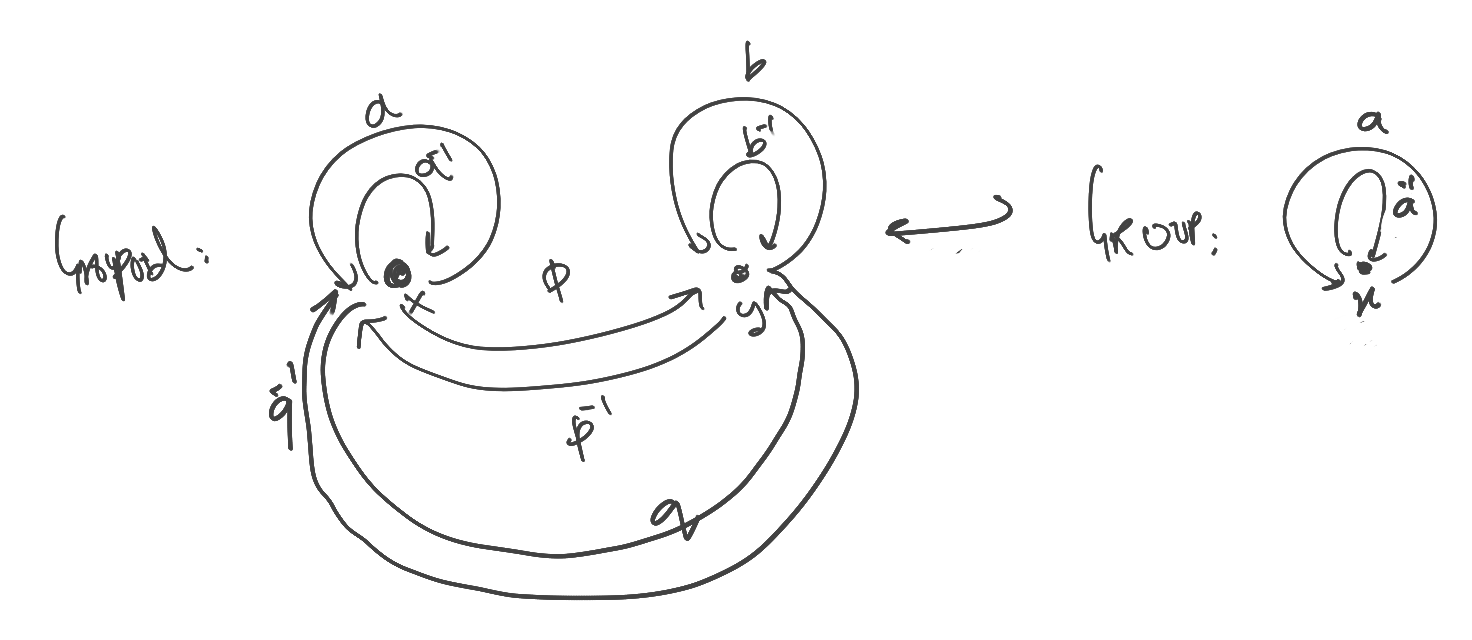
\includegraphics[width=\textwidth]{./groupoid-to-group.png}
\end{frame}

\begin{frame}{Equivalence of categories is Unintuitive (to me)}
    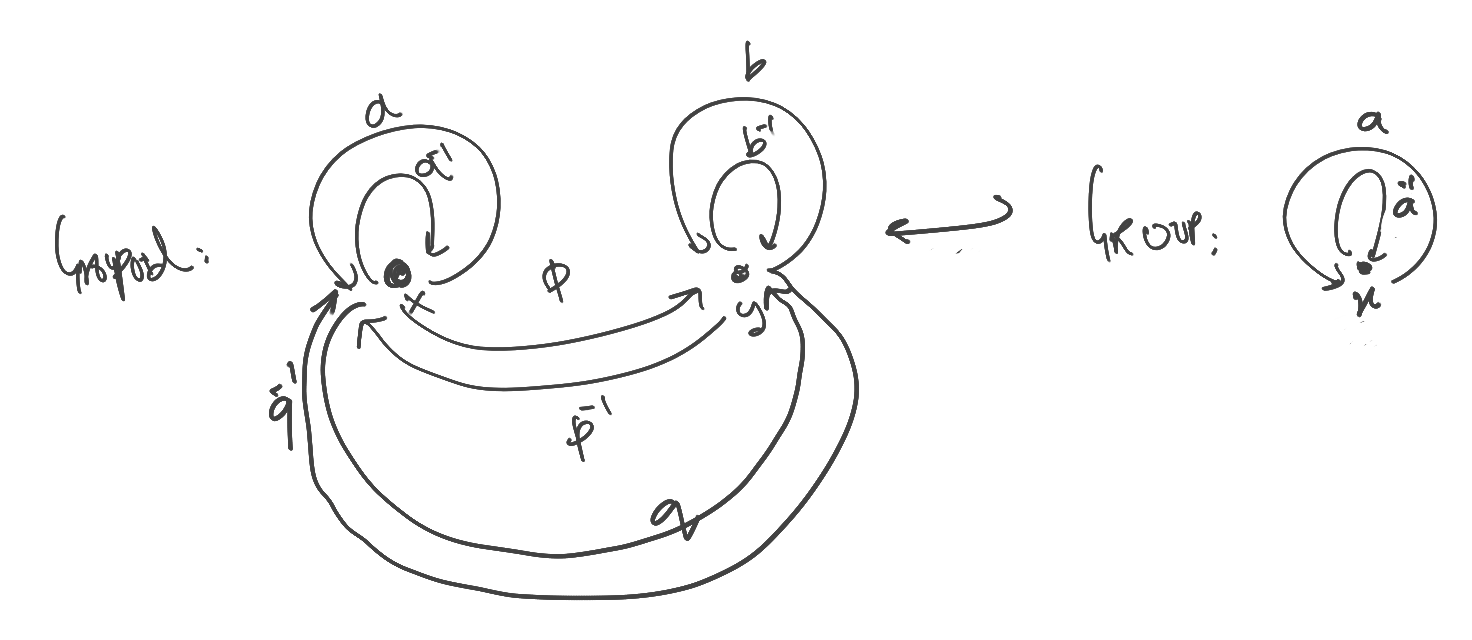
\includegraphics[width=0.7\textwidth]{./groupoid-to-group.png} \pause
    \begin{itemize}
        \item Let $O$ be a connected groupoid, and let $x \in O$ be some  object of the groupoid. Exract out a single object of the groupoid, by considering the subcategory
            consisting of only the object $x \in O$. Label this subcategory $G$. \pause
        \item The embedding functor $F: G \rightarrow O$ is full and faithful since its image contains a single object ($x$) where it preserves all arrows. \pause
        \item Also see that it is essentially surjective. \pause For any other $y \in O$, we have a path $x \xrightarrow{p} y$ (as $O$ is connected). \pause
            \pause since it is a groupoid, all morphisms are isos, and thus $y \simeq x$. \pause
        \item Soo, this is an equivalence of categories?! \pause
        \item Philosophically, equivalence of categories does not need to
            preserve size. \pause It only needs to preserve a ``copy of
            information''. \pause Connected Groupoid contains many copies of
            the same information. \pause It is safe for forget these. \pause
    \end{itemize}
\end{frame}


\begin{frame}{Skeleta}
    \begin{itemize}
        \item A category is \emph{skeletal} iff each isomorphism class has a
        single object.  \pause
    \item $Mat$, category of numbers and materices is the
            skeleton of $\operatorname{FinVectBasis}$, category of finite
            vector spaces with bases, and morphisms as matrices encoding linear
            operators relative to the basis.
        \item Can build $sk(C)$ (Skeleton of $C$). Crush each isomorphism class into a single object.
        \item The inclusion $sk(C) \hookrightarrow C$ defines an equivalence of categories.
    \end{itemize}
\end{frame}


\end{document}
